\section{Desarrollo}
% Metodologia / Desarrollo
Tomando en cuenta que nuestra Poblacion total son las combinaciones de las 18 ciudades tenemos que:  
El total seria $18! = 6,402,373,705,728,000$ posibles combinacioneses, lo cual es un numero muy grande para poder evaluar todas las posibles
soluciones, por lo que se opto por utilizar algoritmos geneticos para poder encontrar una solucion aproximada al problema.

\subsection{Codificación}
Para representar las soluciones del TSP en el contexto de algoritmos genéticos, se utiliza una codificación basada en permutaciones.
Cada cromosoma es una secuencia ordenada de números, donde cada número representa una ciudad específica y su posición en la secuencia 
indica el orden en que se visitan las ciudades.

Usando la lista mostrada en la sección~\ref{lista_ciudades}, un cromosoma podría representarse de la siguiente manera (De Norte a Sur):
\[
[11, 13, 7, 2, 8, 5, 0, 6, 3, 9, 14, 10, 17, 1, 4 ,12, 16, 15]
\]
Esta representación asegura que cada ciudad se visite exactamente una vez, y el recorrido comienza y termina en la ciudad de origen.
Las etiquetas numéricas facilitan la manipulación de las rutas durante las operaciones genéticas como la selección, el cruce y la mutación.

\begin{figure}[H]
    \centering
    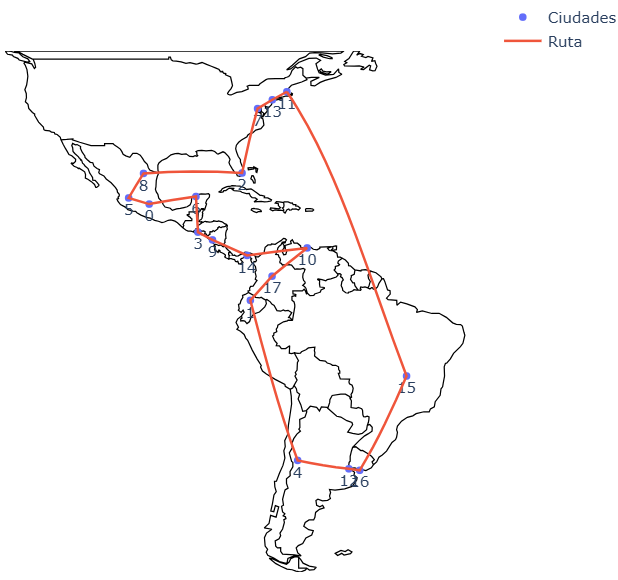
\includegraphics[width=0.75\textwidth]{rsc/img/des/ruta_inicial.png}
    \caption{Ruta propuesta de Norte a Sur para el problema del vendedor viajero.}\label{ruta_inicial}
\end{figure}

Esta ruta solo tiene como objeto una propuesta basada en un analisis visual de las ciudades que nos servira para comparar mas adelante, 
y no representa la mejor ruta posible, ademas de esto debemos tomar en cuenta que el punto de partida puede ser cualquiera de las ciudades, por lo
que la ruta puede variar dependiendo de la ciudad inicial.

\subsection{Generar Población Inicial}
Para generar nuestra población inicial, se crean múltiples cromosomas (rutas) usando la función sample de la librería random 
de python esto nos crea una lista de la longitud deseada sin repetir elementos y en un orden aleatorio, asegurando que cada ciudad se visite 
exactamente una vez en cada ruta.

\begin{figure}[H]
    \centering
    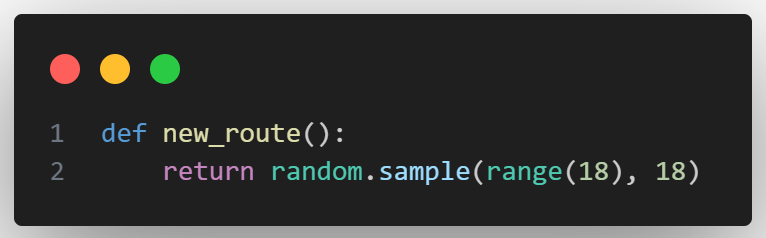
\includegraphics[width=0.65\textwidth]{rsc/img/des/new_rute.png}
    \caption{Funcion generadora de rutas}\label{new_rute}
\end{figure}

\subsection{Evaluar Aptitud}
Como se menciono en la sección~\ref{calculo_distancias}, para evaluar la aptitud de cada cromosoma (ruta), se utiliza la fórmula de Haversine.

Para este problema, tenemos dos opciones: tomar la aptitud de una ruta como el inverso de la distancia total recorrida para buscar maximizar la aptitud,
o simplemente tomar la distancia total como la medida a minimizar siendo este el enfoque mas comun en el TSP es decir tomar la menor aptitud como 
la mejor solucion. En este caso se opto por la segunda opcion.

Una vez entendido esto calculamos la matriz de distancias de Haversine entre todas las ciudades y la almacenamos en una matriz para facilitar 
el calculo de distancias entre ciudades.

\begin{figure}[H]
    \centering
    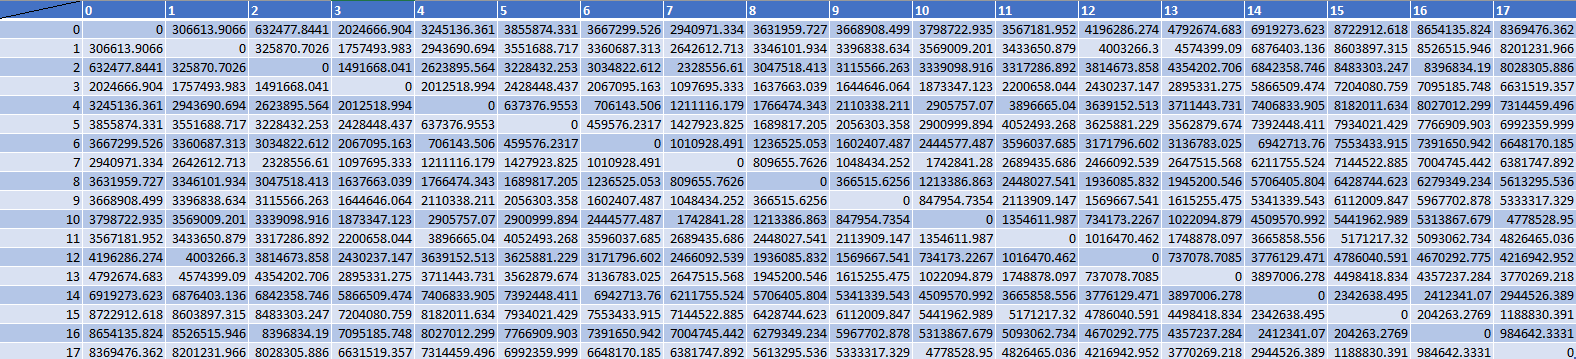
\includegraphics[width=1\textwidth]{rsc/img/des/haversine_matrix.png}
    \caption{Matriz de distancias entre ciudades usando la formula de Haversine}\label{matriz_distancias}
\end{figure}

Como podemos observar en la figura~\ref{matriz_distancias} la matriz es simetrica de ($18\times18$) y la diagonal principal es cero, ya que la distancia de una ciudad
a si misma es cero. Para medir la aptitud de un cromosoma, se calcula la distancia entre cada par de ciudades consecutivas en la ruta, sumando estas
distancias para obtener la distancia total del recorrido.

Con lo anterior podemos generar nuestra poblacion inicial y evaluar su aptitud con la siguiente funcion:

\begin{figure}
    \centering
    
\includegraphics[width=0.65\textwidth]{rsc/img/des/gen_pob.png}
    \caption{Funcion generadora de la poblacion con aptitud}\label{gen_pob}
\end{figure}

\subsection{Ordenar Población}
Para ordenar la población en función de la aptitud de cada cromosoma (ruta), se utiliza la función sorted de Python junto con un reset\_index de 
pandas para reordenar los índices después de la ordenación tomando como clave de ordenación la columna `apt`.

\begin{figure}[H]
    \centering
    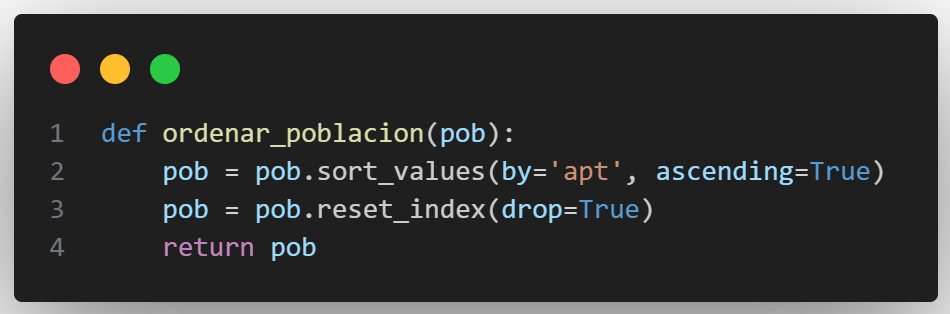
\includegraphics[width=0.65\textwidth]{rsc/img/des/ordenar.png}
    \caption{Funcion para ordenar la poblacion por aptitud}\label{ord_pob}
\end{figure}

\subsection{Selección}

Para la selección de padres en el proceso de cruce, usaremos los metodos de torneo y ranking, para lo cual en cada generacion tomaremos la mitad 
superior de la poblacion ordenada para aplicar rank y la mitad inferior para aplicar torneo, esto con el objetivo de mantener diversidad en la 
poblacion y evitar caer en un minimo local.

\begin{figure}[H]
    \centering
    \begin{subfigure}{0.45\textwidth}
        
\includegraphics[width=1\textwidth]{rsc/img/des/rank.png}
        \caption{Funcion ranking}\label{rank}
    \end{subfigure}
    \hfill
    \begin{subfigure}{0.45\textwidth}
        
\includegraphics[width=1\textwidth]{rsc/img/des/torneo.png}
        \caption{Funcion torneo}\label{torneo}
    \end{subfigure}
    \caption{Funciones de seleccion de padres}\label{seleccion}
\end{figure}

\subsection{Cruce}
Para el cruce de los cromosomas (rutas), se implementaron dos métodos: PMX y PBX.\@

\subsubsection{PMX (Partially Mapped Crossover)}
El cruce PMX selecciona dos padres y se elige un segmento de la ruta de uno de ellos. Luego, se 
mapea este segmento a la ruta del otro padre, asegurando que no se repitan ciudades. Como se explica en la sección~\ref{intro_pmx}.

\begin{figure}[H]
    \centering
    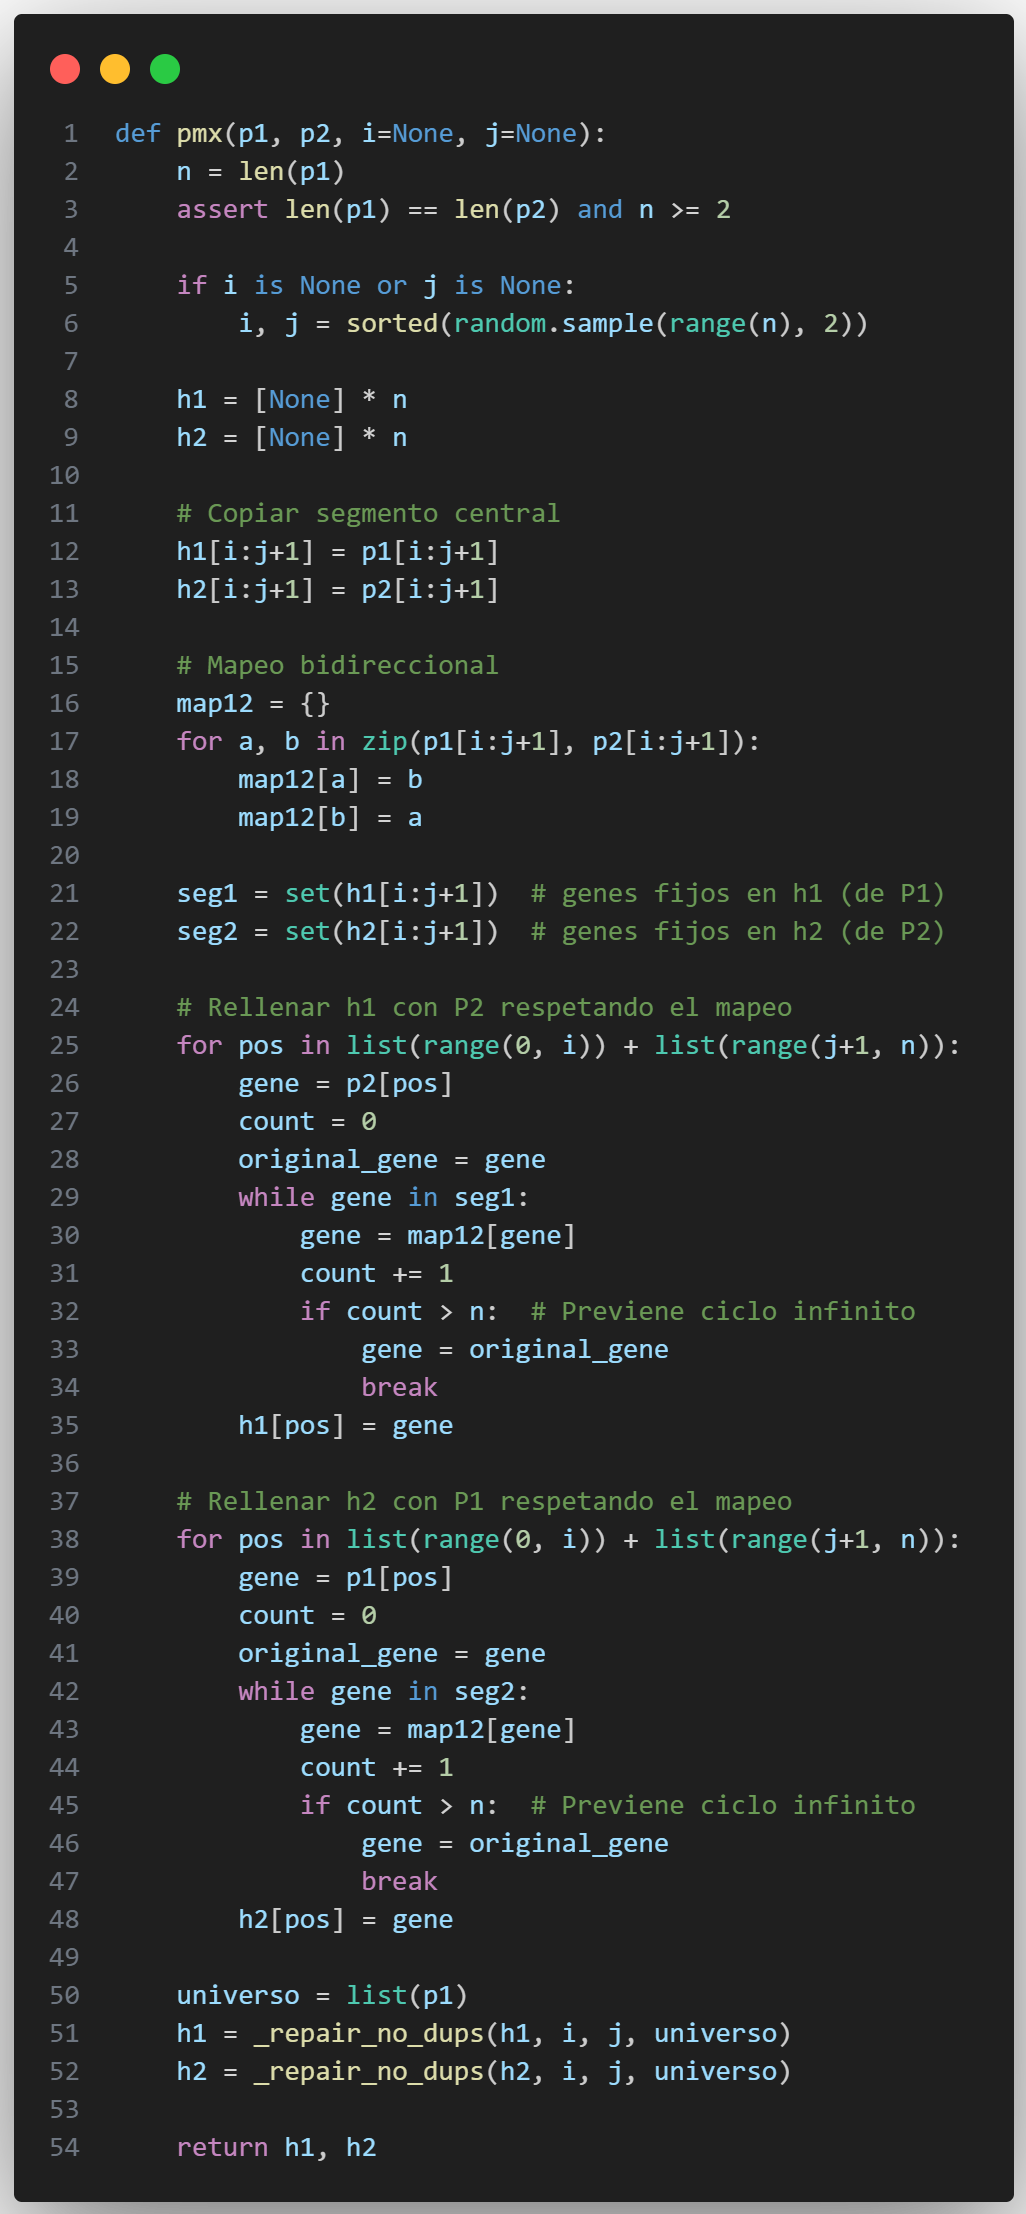
\includegraphics[width=0.45\textwidth]{rsc/img/des/pmx.png}
    \caption{Funcion de cruce PMX}\label{pmx}
\end{figure}

\subsubsection{PBX (Position-Based Crossover)}
El cruce PBX selecciona aleatoriamente varias posiciones en la ruta de un padre y copia las ciudades en esas posiciones al hijo. Luego,
completa las posiciones restantes con las ciudades del otro padre, manteniendo el orden relativo. Este se explica en la sección~\ref{intro_pbx}.

\begin{figure}[H]
    \centering
    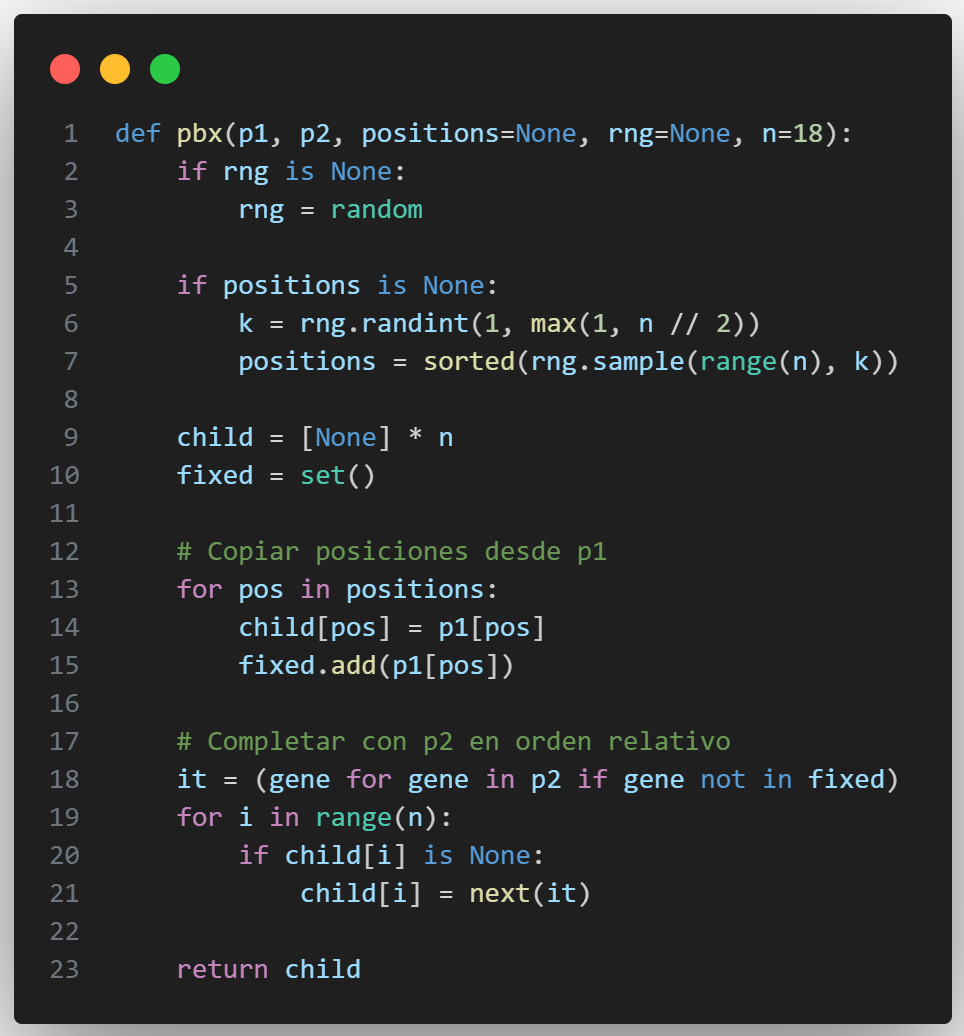
\includegraphics[width=0.65\textwidth]{rsc/img/des/pbx.png}
    \caption{Funcion de cruce PBX}\label{pbx}
\end{figure}

\subsection{Mutación}

Para la mutación de las rutas, se implementaron dos métodos: mezcla (scramble) e intercambio de bloques (block transpose).\@

\subsubsection{Mutación de Mezcla (Scramble Mutation)}
La mutación de mezcla selecciona un segmento aleatorio de la ruta y reordena las ciudades dentro de ese segmento de manera aleatoria.

\begin{figure}[H]
    \centering
    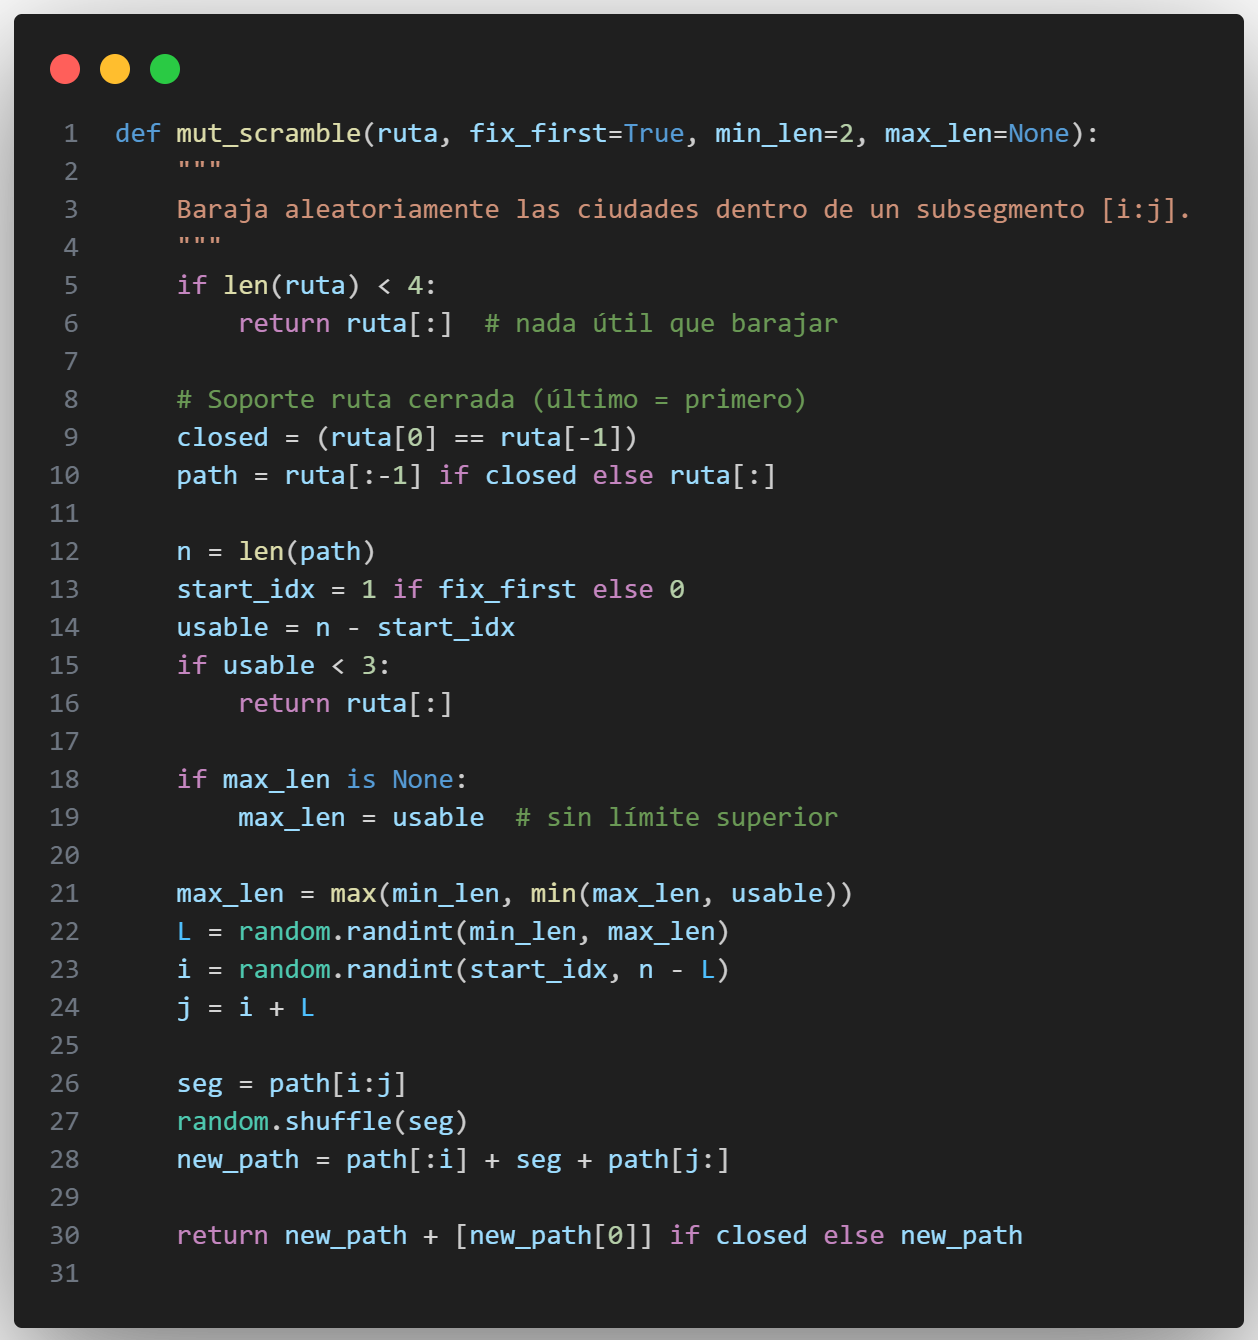
\includegraphics[width=0.5\textwidth]{rsc/img/des/scramble.png}
    \caption{Funcion de mutacion scramble}\label{scramble}
\end{figure}

\subsubsection{Mutación de Intercambio de Bloques (Block Transpose Mutation)}

La mutación de intercambio de bloques selecciona dos segmentos de la ruta y los intercambia entre sí.

\begin{figure}[H]
    \centering
    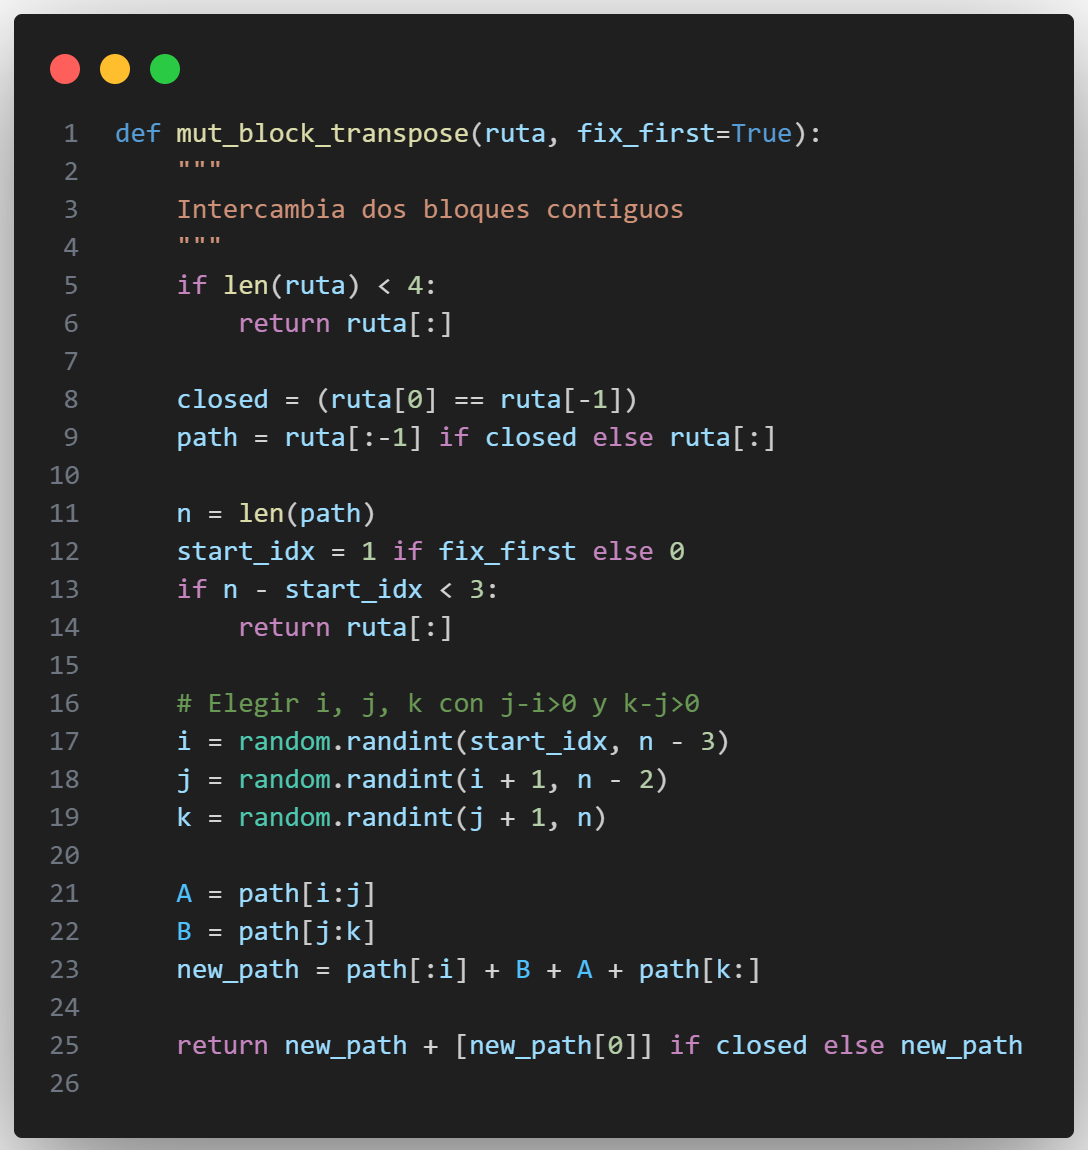
\includegraphics[width=0.5\textwidth]{rsc/img/des/block_transpose.png}
    \caption{Funcion de mutacion block transpose}\label{block_transpose}
\end{figure}

\subsection{Ejecucion del Algoritmo Genético}

Por ultimo, se implementa la función principal del algoritmo genético que integra todos los componentes anteriores. Esta función parte de una población inicial,
N generaciones y tipo de cruce ademas de ofrecernos una grafica con el progreso de la mejor solución encontrada. De manera interna se selecciona el tipo de mutacion 
si se estanca la poblacion.

\begin{figure}[H]
    \centering
    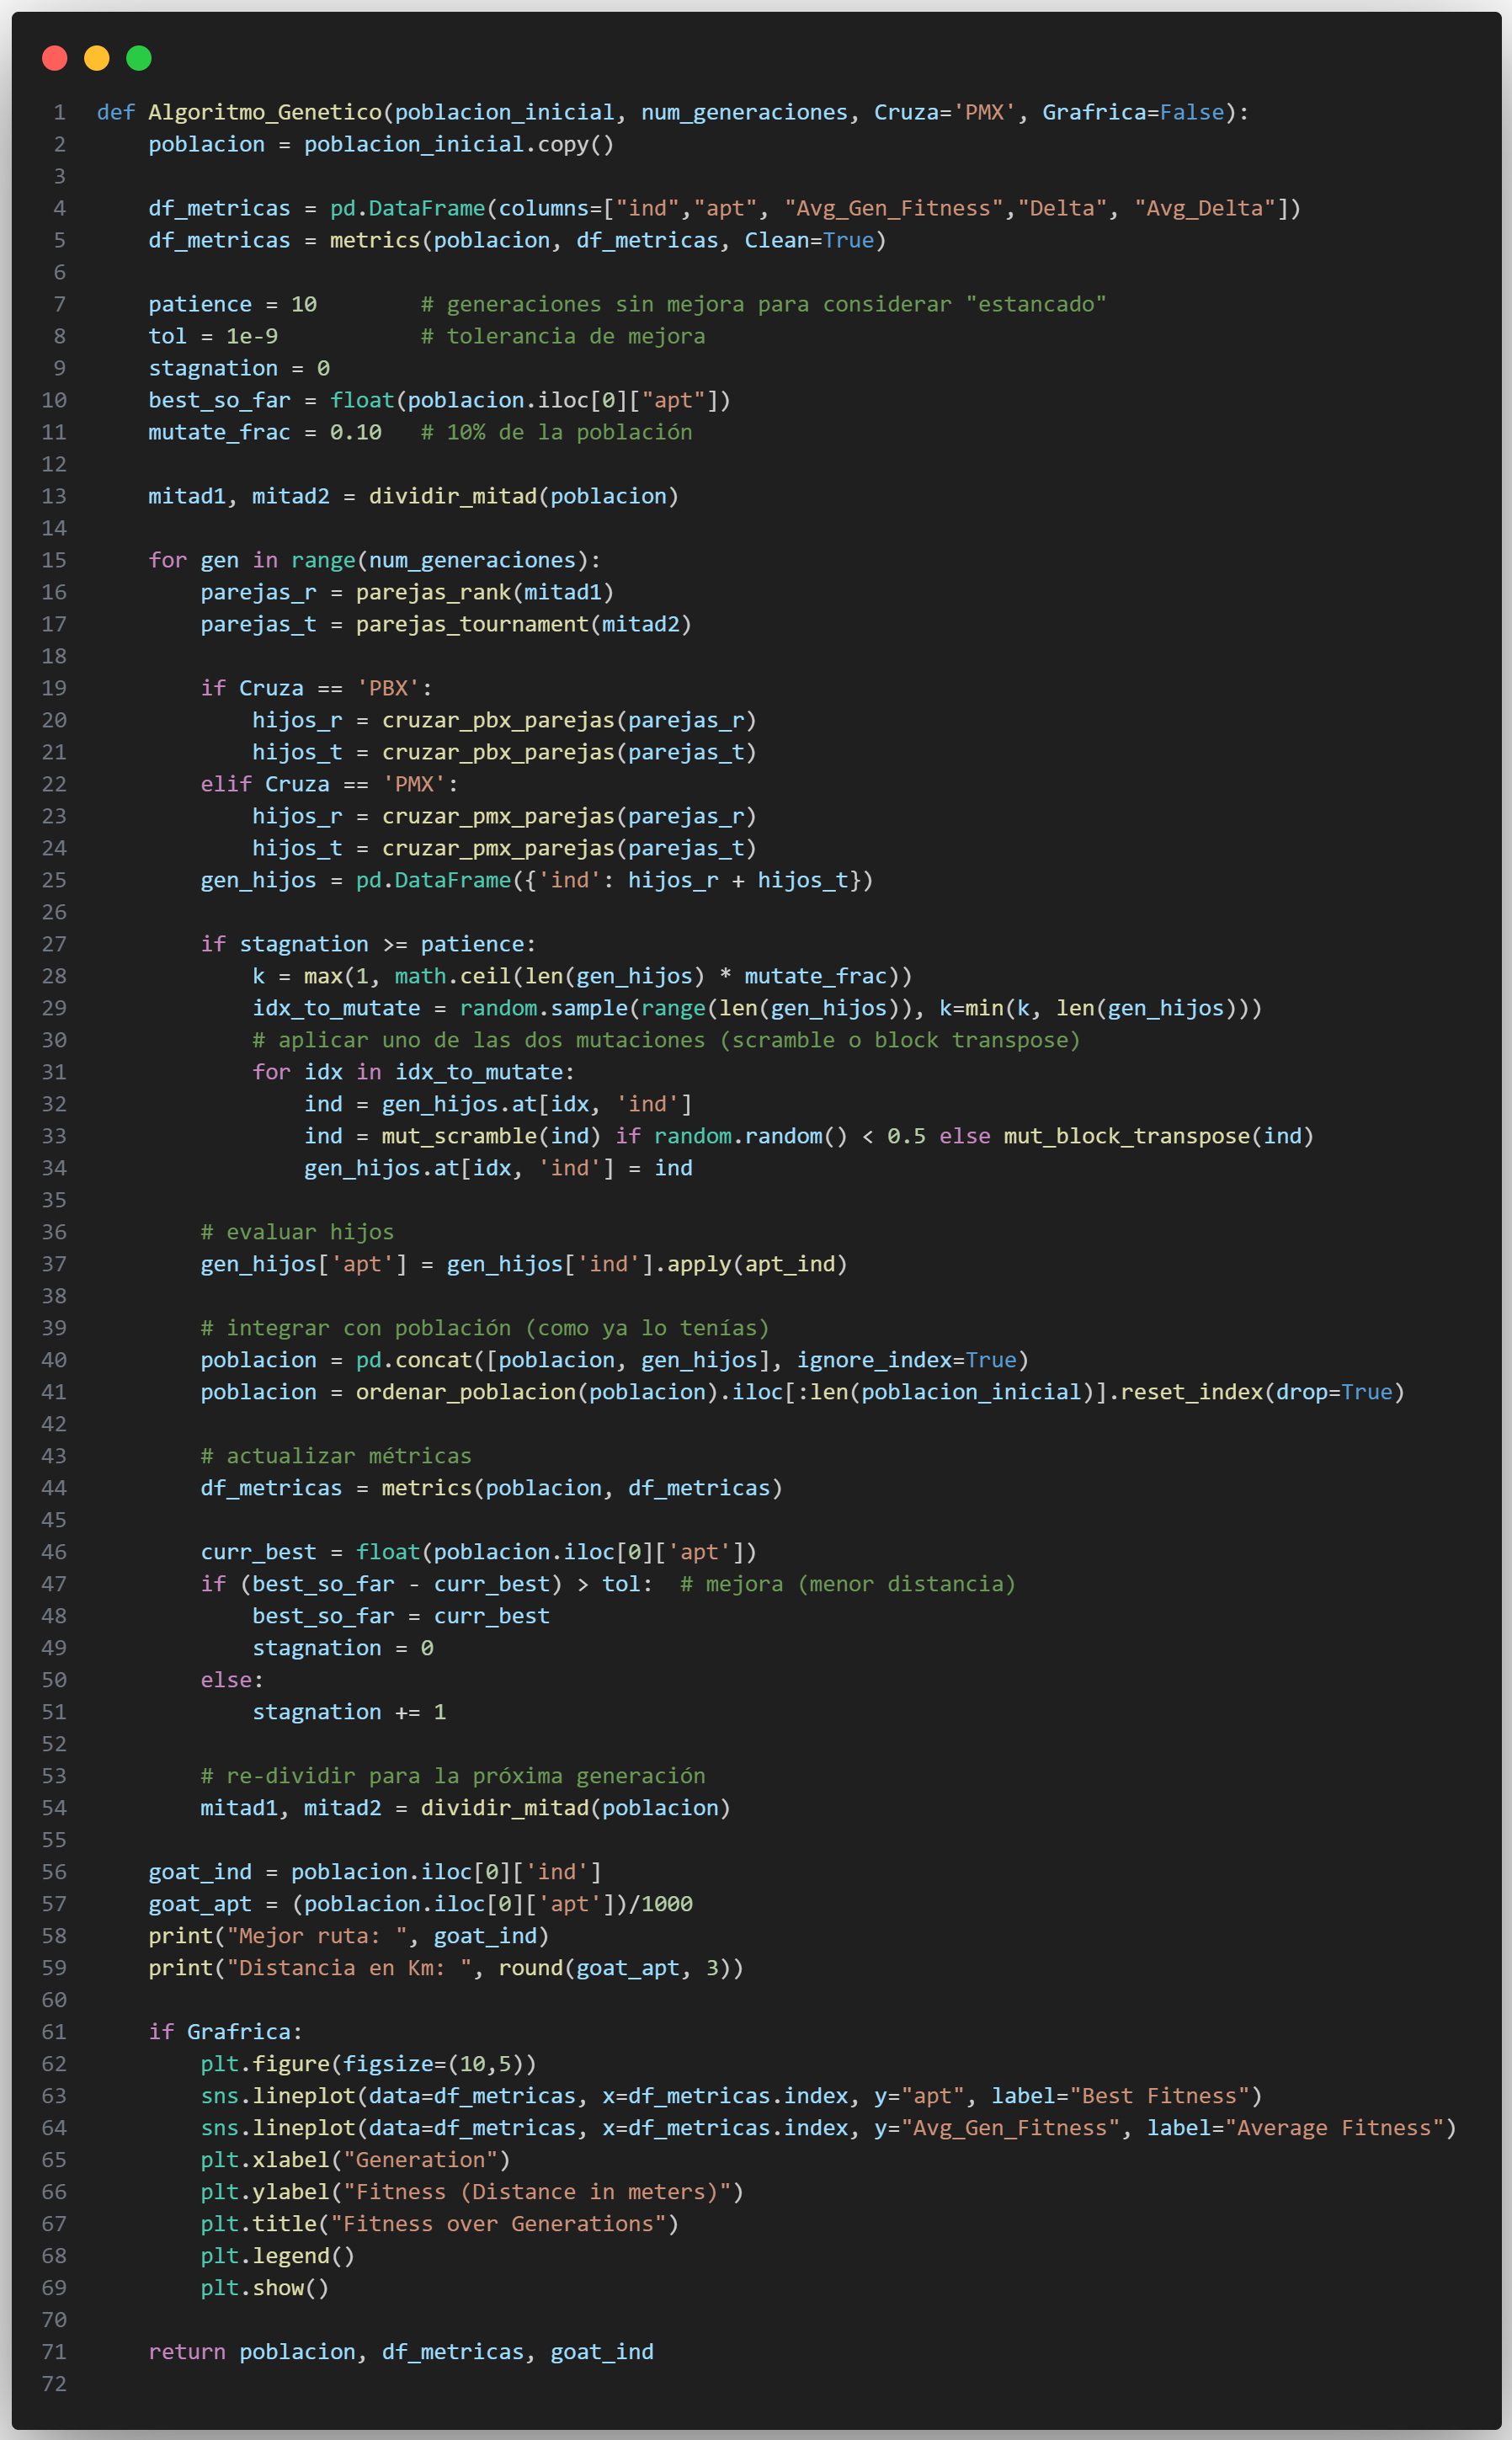
\includegraphics[width=0.65\textwidth]{rsc/img/des/alg_gen.png}
    \caption{Funcion principal del algoritmo genetico}\label{alg_genetico}
\end{figure}

Con esta función, ejecutamos nuestro algoritmo genético para encontrar una solución aproximada al problema del vendedor viajero para lo cual
usamos 4 Poblaciones iniciales diferentes con nuestros 2 tipos de cruce y 1000 generaciones cada una, con el objetivo de comparar resultados 
y observar la convergencia del algoritmo. Cabe mencionar que las poblaciones iniciales fueron generadas de manera aleatoria pero se mantienen
constantes para cada corrida del algoritmo de manera que nuestra comparacion sea valida.

\subsection{Poblacion Inicial: 100} %%%%%%%%%%%%%%%%%%%%%%%%%%%%%%%%%%%%%%%%%%%%%%%%%%%%%%%%%%

\subsubsection{Cruce PMX}\label{100_pmx}

Mejor ruta:  [6, 2, 7, 13, 11, 10, 15, 16, 12, 4, 1, 17, 14, 9, 3, 0, 5, 8]

Distancia en Km:  23,987.019

\begin{figure}[H]
    \centering
    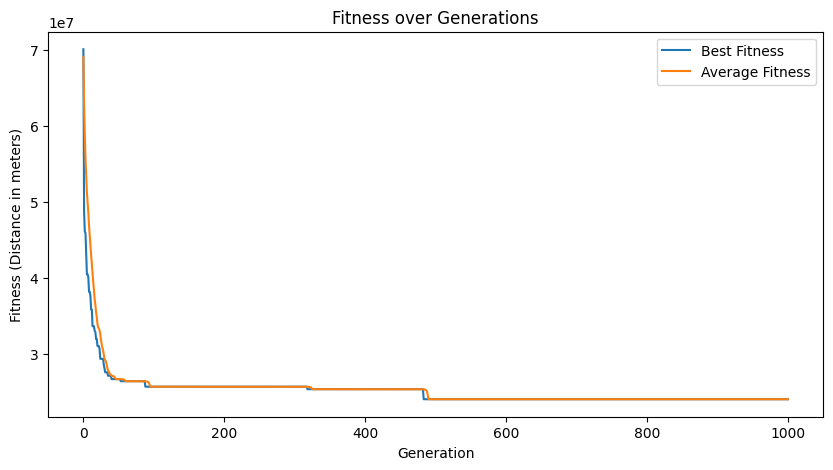
\includegraphics[width=0.75\textwidth]{rsc/img/des/Metrics_100_pmx.png}
    \caption{Evolucion de la mejor aptitud con cruce PMX y poblacion inicial 100}\label{Metrics_100_pmx}
\end{figure}

\begin{figure}[H]
    \centering
    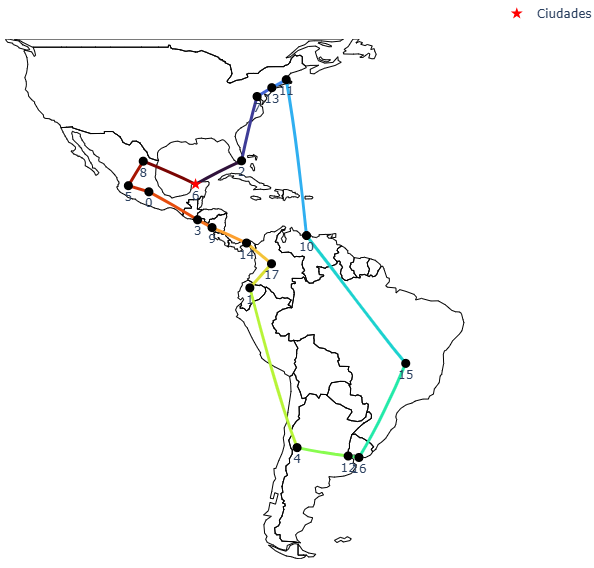
\includegraphics[width=0.65\textwidth]{rsc/img/des/ruta_100_pmx.png}
    \caption{Mejor ruta encontrada con cruce PMX y poblacion inicial 100}\label{ruta_100_pmx}
\end{figure}

\subsubsection{Cruce PBX}\label{100_pbx}
Mejor ruta:  [15, 16, 12, 4, 1, 17, 14, 9, 3, 6, 0, 5, 8, 7, 13, 11, 2, 10]

Distancia en Km:  24,052.637

\begin{figure}[H]
    \centering
    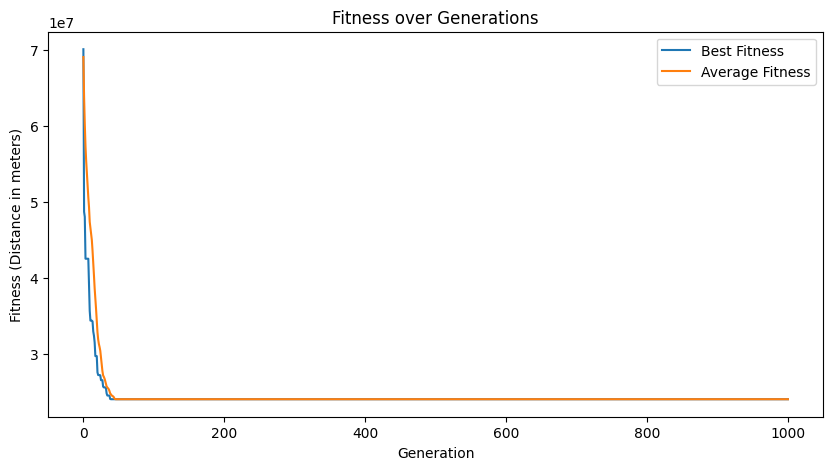
\includegraphics[width=0.75\textwidth]{rsc/img/des/Metrics_100_pbx.png}
    \caption{Evolucion de la mejor aptitud con cruce PBX y poblacion inicial 100}\label{Metrics_100_pbx}
\end{figure}
\begin{figure}[H]
    \centering
    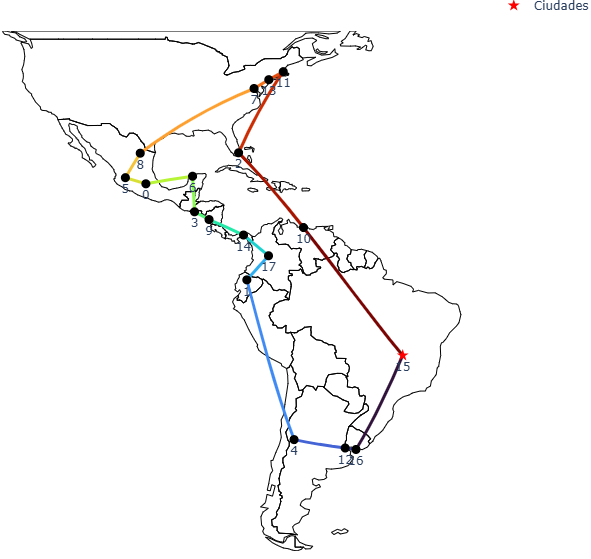
\includegraphics[width=0.65\textwidth]{rsc/img/des/ruta_100_pbx.png}
    \caption{Mejor ruta encontrada con cruce PBX y poblacion inicial 100}\label{ruta_100_pbx}
\end{figure}

\subsection{Poblacion Inicial: 200} %%%%%%%%%%%%%%%%%%%%%%%%%%%%%%%%%%%%%%%%%%%%%%%%%%%%%%%%%%

\subsubsection{Cruce PMX}\label{200_pmx}

Mejor ruta:  [2, 6, 8, 5, 0, 3, 9, 14, 17, 1, 4, 12, 16, 15, 10, 11, 13, 7]

Distancia en Km:  23,987.019

\begin{figure}[H]
    \centering
    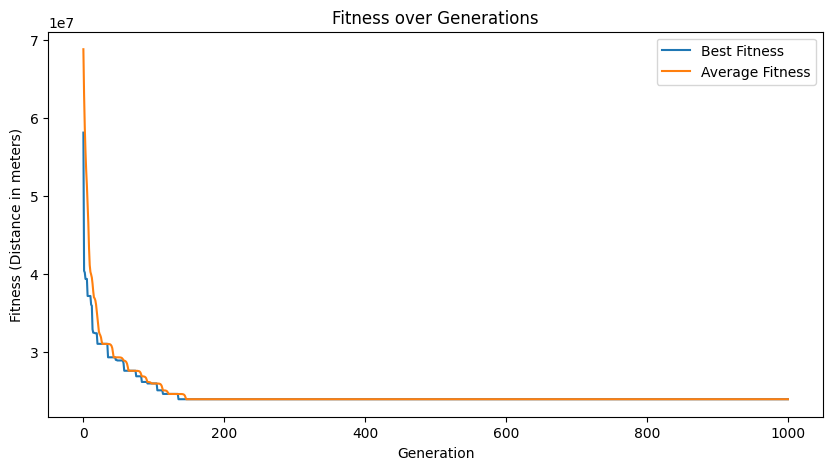
\includegraphics[width=0.75\textwidth]{rsc/img/des/Metrics_200_pmx.png}
    \caption{Evolucion de la mejor aptitud con cruce PMX y poblacion inicial 200}\label{Metrics_200_pmx}
\end{figure}

\begin{figure}[H]
    \centering
    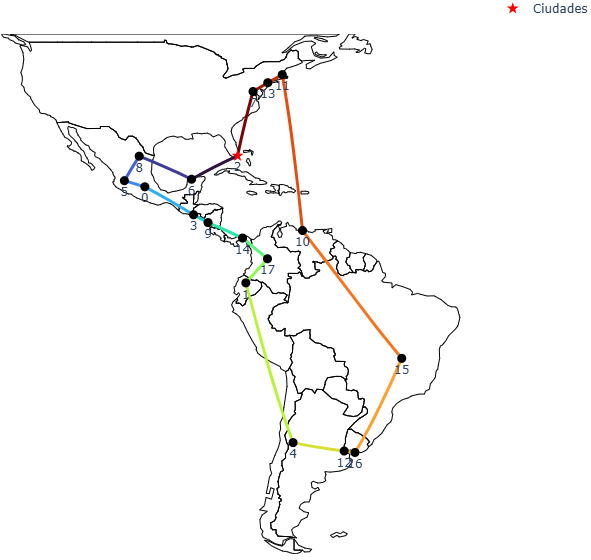
\includegraphics[width=0.65\textwidth]{rsc/img/des/ruta_200_pmx.png}
    \caption{Mejor ruta encontrada con cruce PMX y poblacion inicial 200}\label{ruta_200_pmx}
\end{figure}

\subsubsection{Cruce PBX}\label{200_pbx}

Mejor ruta:  [8, 5, 0, 6, 3, 9, 1, 4, 12, 16, 15, 10, 17, 14, 2, 11, 13, 7]

Distancia en Km:  24,772.018

\begin{figure}[H]
    \centering
    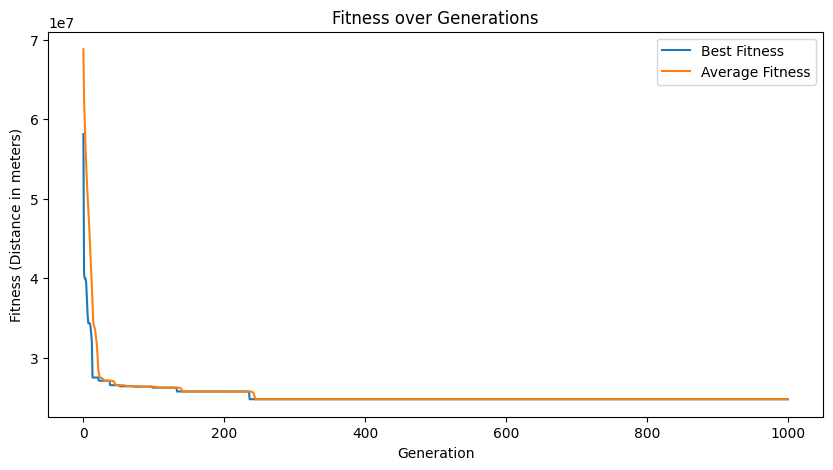
\includegraphics[width=0.75\textwidth]{rsc/img/des/Metrics_200_pbx.png}
    \caption{Evolucion de la mejor aptitud con cruce PBX y poblacion inicial 200}\label{Metrics_200_pbx}
\end{figure}

\begin{figure}[H]
    \centering
    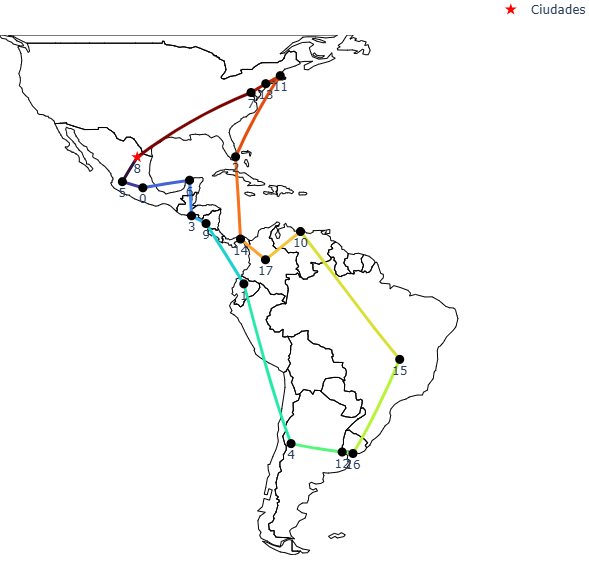
\includegraphics[width=0.65\textwidth]{rsc/img/des/ruta_200_pbx.png}
    \caption{Mejor ruta encontrada con cruce PBX y poblacion inicial 200}\label{ruta_200_pbx}
\end{figure}

\subsection{Poblacion Inicial: 500} %%%%%%%%%%%%%%%%%%%%%%%%%%%%%%%%%%%%%%%%%%%%%%%%%%%%%%%%%%

\subsubsection{Cruce PMX}\label{500_pmx}
Mejor ruta:  [6, 2, 7, 13, 11, 10, 15, 16, 12, 4, 1, 17, 14, 9, 3, 0, 5, 8]

Distancia en Km:  23,987.019

\begin{figure}[H]
    \centering
    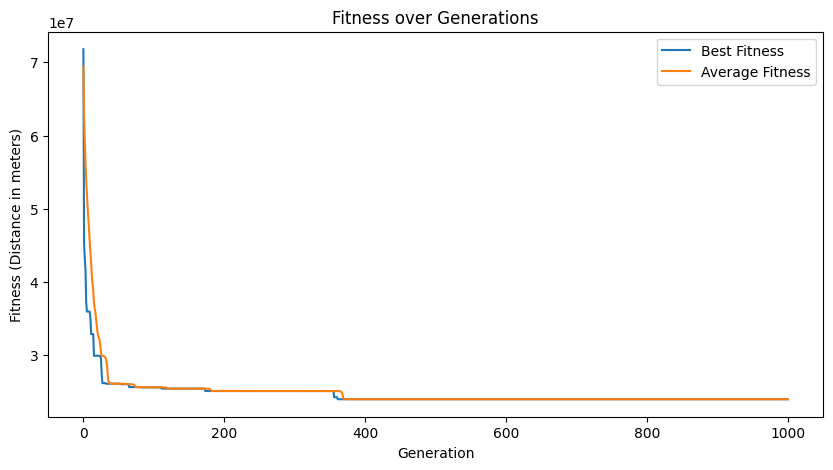
\includegraphics[width=0.75\textwidth]{rsc/img/des/Metrics_500_pmx.png}
    \caption{Evolucion de la mejor aptitud con cruce PMX y poblacion inicial 500}\label{Metrics_500_pmx}
\end{figure}

\begin{figure}[H]
    \centering
    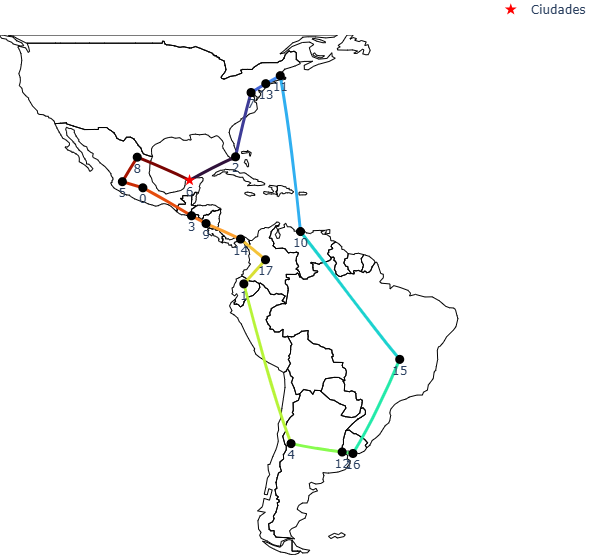
\includegraphics[width=0.65\textwidth]{rsc/img/des/ruta_500_pmx.png}
    \caption{Mejor ruta encontrada con cruce PMX y poblacion inicial 500}\label{ruta_500_pmx}
\end{figure}

\subsubsection{Cruce PBX}\label{500_pbx}
Mejor ruta:  [12, 16, 15, 10, 2, 11, 13, 7, 8, 5, 0, 6, 3, 9, 14, 17, 1, 4]

Distancia en Km:  24,052.637

\begin{figure}[H]
    \centering
    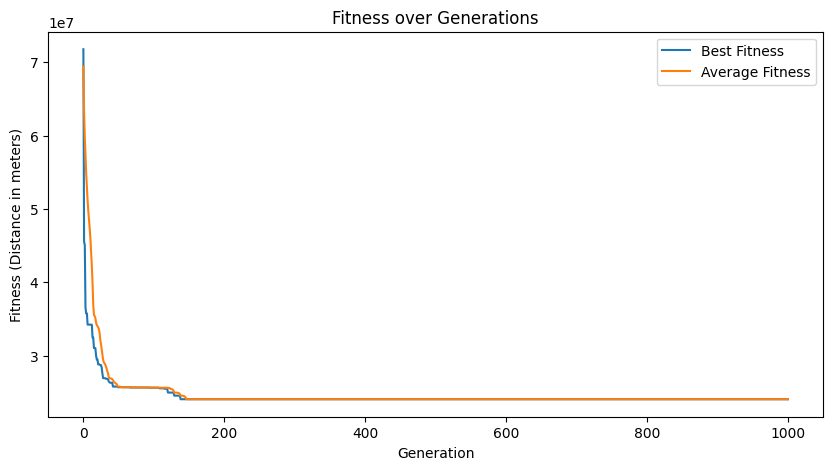
\includegraphics[width=0.75\textwidth]{rsc/img/des/Metrics_500_pbx.png}
    \caption{Evolucion de la mejor aptitud con cruce PBX y poblacion inicial 500}\label{Metrics_500_pbx}
\end{figure}

\begin{figure}[H]
    \centering
    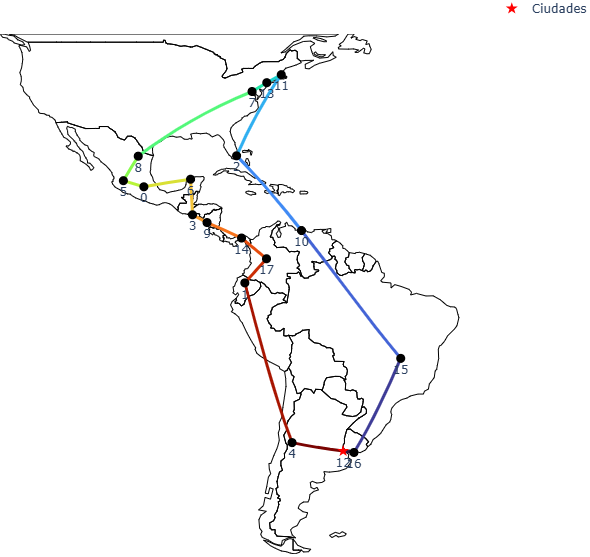
\includegraphics[width=0.65\textwidth]{rsc/img/des/ruta_500_pbx.png}
    \caption{Mejor ruta encontrada con cruce PBX y poblacion inicial 500}\label{ruta_500_pbx}
\end{figure}

\subsection{Poblacion Inicial: 1000} %%%%%%%%%%%%%%%%%%%%%%%%%%%%%%%%%%%%%%%%%%%%%%%%%%%%%%%%%%
\subsubsection{Cruce PMX}\label{1000_pmx}
Mejor ruta:  [12, 16, 15, 10, 2, 11, 13, 7, 8, 5, 0, 6, 3, 9, 14, 17, 1, 4]

Distancia en Km:  24,052.637

\begin{figure}[H]
    \centering
    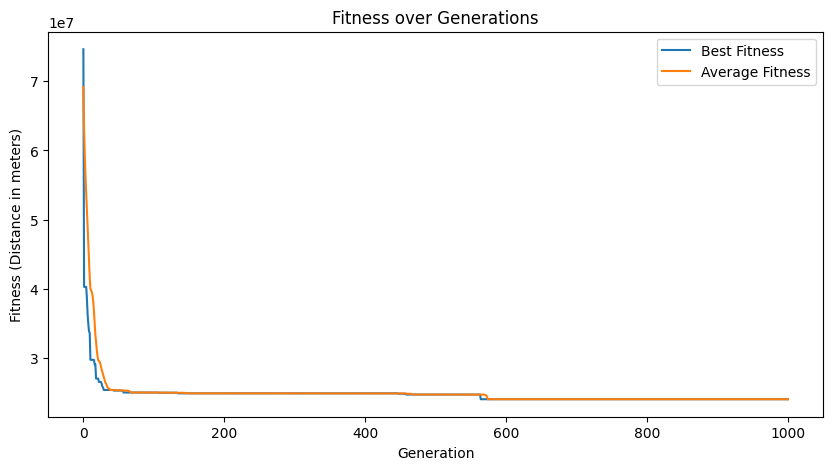
\includegraphics[width=0.75\textwidth]{rsc/img/des/Metrics_1000_pmx.png}
    \caption{Evolucion de la mejor aptitud con cruce PMX y poblacion inicial 1000}\label{Metrics_1000_pmx}
\end{figure}

\begin{figure}[H]
    \centering
    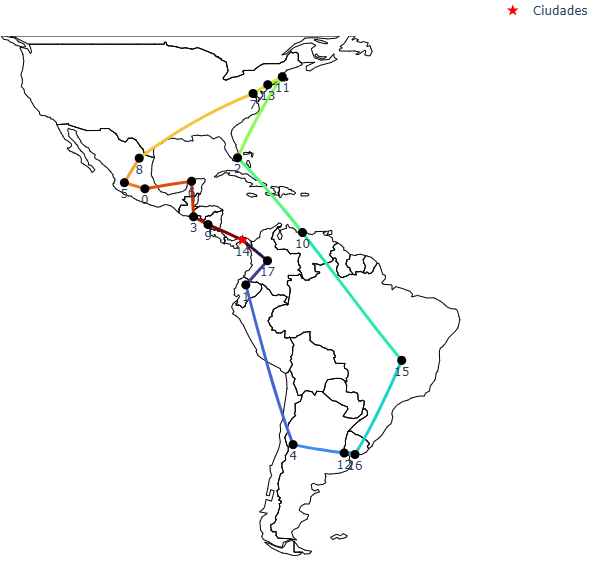
\includegraphics[width=0.65\textwidth]{rsc/img/des/ruta_1000_pmx.png}
    \caption{Mejor ruta encontrada con cruce PMX y poblacion inicial 1000}\label{ruta_1000_pmx}
\end{figure}

\subsubsection{Cruce PBX}\label{1000_pbx}
Mejor ruta:  [16, 15, 10, 17, 14, 2, 11, 13, 7, 8, 5, 0, 6, 3, 9, 1, 4, 12]

Distancia en Km:  24,772.018

\begin{figure}[H]
    \centering
    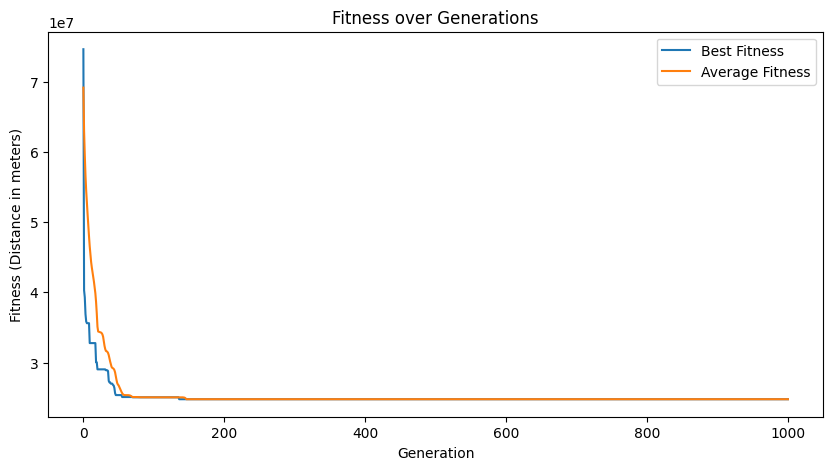
\includegraphics[width=0.75\textwidth]{rsc/img/des/Metrics_1000_pbx.png}
    \caption{Evolucion de la mejor aptitud con cruce PBX y poblacion inicial 1000}\label{Metrics_1000_pbx}
\end{figure}

\begin{figure}[H]
    \centering
    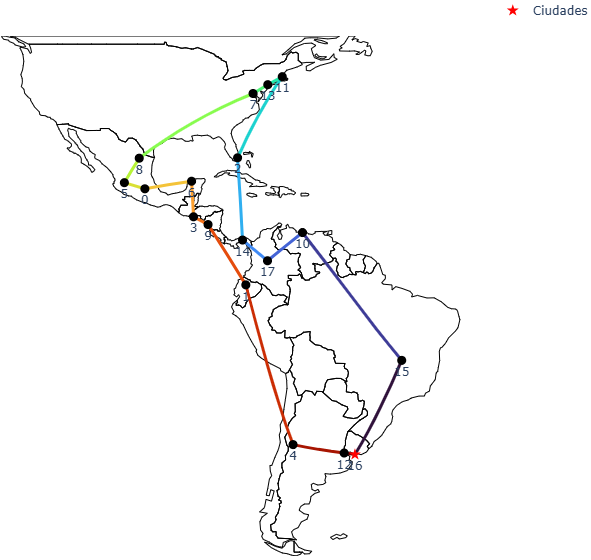
\includegraphics[width=0.65\textwidth]{rsc/img/des/ruta_1000_pbx.png}
    \caption{Mejor ruta encontrada con cruce PBX y poblacion inicial 1000}\label{ruta_1000_pbx}
\end{figure}
